\documentclass{article}
\usepackage[T1]{fontenc}
\usepackage[utf8]{inputenc}
\usepackage{geometry}
\usepackage{amsmath}
\usepackage{algorithm}
\usepackage{algpseudocode}
\usepackage{graphicx}
\usepackage{booktabs}
\usepackage{pdflscape}
\usepackage[export]{adjustbox}
\geometry{a4paper,tmargin=1in,bmargin=1in,lmargin=0.95in,rmargin=0.95in}

\usepackage[sorting=none]{biblatex}
\addbibresource{references.bib}

\title{15-418/516 Final Project: Parallel-In-Time Integration}
\author{Alexius Wadell (awadell)}
\date{\today}

\usepackage{setspace}
\setstretch{1.5}

\begin{document}

\maketitle

\section{Summary}
For my project, I implemented the Multigrid Reduction in Time (MGRIT) and Parareal algorithms for solving ordinary differential equations using the threading primitives provided by the Julia Programming Language.
I then benchmarked both algorithms on both my 2020 Macbook Pro (M1 chip), and my group's cluster (AMD EPYC 7713 64-Core Processor).
Overall, the overhead of Julia's threading primitives limited the speedup on small problems, but for a sufficiently expensive differential, I was able to achieve notable speedups over a serial implementation on both systems.

Throughout this project, I learned a lot about applying the concepts from the course to debugging and understanding the performance limitations of Julia's threading primitives.
While the tools presented in class (OpenMP, CUDA, AVX) were extremely transparent, and thus complex to use, the primitives provided by Julia were both simple and opaque.
Unfortunately, this made it difficult to deceiver what exactly was happening under the hood.

\section{Background}

Solving ordinary differential equations (ODE) numerically is generally done using by incremental stepping forwards in time.
For example, given a differential equation (Eq.~\ref{eq:differential}) and initial conditions \( u(0) = u_0 \), we can step forward in using Euler's method (Eq.~\ref{eq:euler}).

\begin{equation}\label{eq:differential}
    \frac{du}{dt} = f(u, t)
\end{equation}

\begin{equation}\label{eq:euler}
    u(t + dt) = u(t) + \delta t \cdot f(u(t), t)
\end{equation}

More generally, a set of discrete time points \( t = i \delta t \) for \( i = 0,1,2,\dots N\), and some serial integrator \( \Phi(u_i) = u_{i+1} \), we want to find \( u_i\) for \( i \in [1, N] \).
One of the benefits of the MGRIT algorithm is that we can use any serial integrator for \(\Phi\).
For example, using Euler's method, \( \Phi(u_i) = u_i + \delta t f(u_i, t) \).
By leveraging, DifferentialEquations.jl~\cite{rackauckasDifferentialEquationsJlPerformant2017a}, I was able to easily take advantage of a wide range of serial integrators.
For the sake of this project, I have used the \verb!Tsit5! integrator, a fourth-order Runge-Kutta method developed by \citeauthor{tsitouras2011runge}.

Typically, solving an ODE is done by iteratively applying a serial integrator to set forward in time, resulting in a cost that is linear in the number of time steps.
As each step is dependent on the last, there is no obvious method for paralleling over time.
Instead, most work has focused on parallelization within the differential \(f\), with most intergrator suites lacking any parallel-in-time capabilities~\cite{ComparisonDifferentialEquation2017}.

In this project, I have implemented two parallel-in-time algorithms for solving ODEs: Parareal\cite{lionsResolutionEDPPar2001} and MGRIT\cite{friedhoffMULTIGRIDINTIMEALGORITHMSOLVING}.
The Parareal Algorithm, iteratively applies a ``coarse'' integrator to predict the state at some coarse time step(\( t\delta \)), and a ``fine'' integrator to refine the prediction between coarse time steps in parallel.
This is repeated until convergence is achieved, which for \(N_c\) coarse time steps will occur in at most \(N_c\) iterations~\cite{lionsResolutionEDPPar2001}.
As after \(N_c\) iterations, we have effectively applied the fine integrators in serial.
Of course, in order to achieve speedup we must converge in less than \(N_c\) iterations, ideally significantly less.
As such, the usefulness Parareal algorithm is limited to problems that require very high accuracy, but can also be well approximated using a coarse integrator.
As such, it's implementation here was mostly as a stepping stone to MGRIT.

The Multigrid Reduction in Time (MGRIT) algorithm reframes solving an ODE as solving a large diagonal system of linear equations, and is currently being developed into the XBraid package by Lawrence Livermore National Laboratory~\cite{xbraid-package}.
Specifically, MGRIT is trying to solve the linear system of equations \( A u = g \) given by Eq.~\ref{eq:mgrit}.
Where \( g_0 = u_0\), and \( \Phi \) is the linear realization of the serial integrator (i.e. \( \Phi(u) \equiv \Phi \cdot u \)).
From here, the MGRIT algorithm now treats ``time'' as an additional spatial dimension, and proceeds to solve it using existing multigrid reduction methods.
That is, instead of solving the entire system, we solve segments of the solution on a fine grid, and use the coarse grid to rectify the various sub-segments.

\begin{equation}\label{eq:mgrit}
    A u = g \to
    \begin{bmatrix}
    I &  &  &  \\
    -\Phi & I & &  \\
    & \ddots  & \ddots  &  \\
    &  & -\Phi & I
   \end{bmatrix}
   \begin{bmatrix}
   u_0 \\
   u_1 \\
   \vdots \\
   u_N
   \end{bmatrix}
   =
   \begin{bmatrix}
   g_0 \\
   g_1 \\
   \vdots \\
   g_N
   \end{bmatrix}
\end{equation}

\begin{figure}
    \centering
    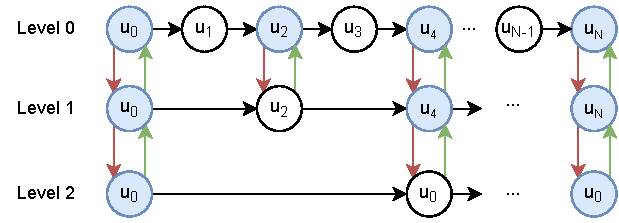
\includegraphics[width=\linewidth]{docs/assets/mgrit_cycle.pdf}
    \caption{MGRIT Algorithm\label{fig:mgrit}}
\end{figure}

Practically, this is done using the algorithm outlined in Algorithm~\ref{alg:mgrit} and Figure~\ref{fig:mgrit}.
But a high level it, we partition the time domain \(t = i \delta t\) into C-points \(i = jm\) (Blue) and F-points (White),
where \(m\) is some coarsening factor, and is typically set to be 2.
We then update each F-point using \(\Phi\) and stepping forward from the previous C-point, this is done in parallel and is called an F-relaxation.
Next we update each C-point using \(\Phi\) and stepping forward from the proceeding F-point, this is also done in parallel and is called an C-relaxation.
An additional F-relaxation is then performed completing the FCF-cycle.
The C-points of the current level are then used to update the next level's point (Red Arrows), and we recurse into the next level.
After updating the coarser levels, we then update the current level's C-Points based on the next level (Green Arrows) and perform a F-relaxation to update the F-points.
This is repeated until convergence is achieved.

As noted by \citeauthor{friedhoffMULTIGRIDINTIMEALGORITHMSOLVING}, the Parareal algorithm is MGRIT restricted to only 2 levels, and using a single F-relaxation, instead of the FCF-cycle used in MGRIT.

\begin{algorithm}[h]
    \caption{The MGRIT Algorithm}\label{alg:mgrit}
    \begin{algorithmic}

        \If{ Current level $l$ is the Coarsest Level}
            \State Solve the system serially: $A_L u_L = g_L$
        \Else
            \State Update the current level using an FCF relaxation
            \For{$j = 0, 1, \dots N_l/m$}  \Comment{In-Parallel F-Relaxation}
                \State Update the F-points: $u_{i+1} = \Phi(u_i) + g_i$
            \EndFor
            \For{$j = 1, \dots N_l/m$}  \Comment{In-Parallel C-Relaxation}
                \State Update the C-Points: $u_{mj} = \Phi(u_{mj-1}) + g_{mj-1}$
            \EndFor
            \For{$j = 0, 1, \dots N_l/m$}  \Comment{In-Parallel F-Relaxation}
                \State Update the F-points: $u_{i+1} = \Phi(u_i) + g_i$
            \EndFor

            \State Inject the residuals of the current level into the next level: $\vec{g}_{l+1} = R_I(\vec{g}_l - A_l \vec{u}_l)$
            \State Solve the next coarse level: $MGRIT(l+1)$
            \State Refine this level using the coarse solution: $\vec{u}_l = \vec{u}_l + P_{\Phi} \vec{u}_{l+1})$
        \EndIf
    \end{algorithmic}
\end{algorithm}

\section{Approach}

For this project, I used the Julia Programming Language\cite{Julia-2017} to implement the MGRIT algorithm on a Shared Memory machine using Julia's built-in threading primitives.
I choose to implement this project using Julia largely due the strength of it's ecosystem for Differential Equations~\cite{rackauckasDifferentialEquationsJlPerformant2017a}.
Hardware-wise, I decided to benchmark my implementation on my 2020 MacBook Pro (M1 Chip) and on the AMD EPYC 7713 64-Core Processor available via the RM nodes on the Bridges2~\cite{Bridges2} or Arjuna~\cite{ArjunaComputingCluster} computing clusters.
Ultimately, this project was guide by my research interest (Modeling Dynamical Systems) and the types of hardware and software I typically use.

\subsection{Data Structures}
I used preallocated vectors of vectors (\verb!Vector{Vector{uType}}!) for storing the solution \(u\), residuals \(g\), and a scratch space for computing the updates to each level.
Additionally, as some integrators \(\Phi\) require additional storage, I preallocated a separate integrator for each thread.
From there it was largely a matter of looping over F/C-points, performing the F/C-relaxations, and then recursing into the next level.

\subsection{Thread Overhead}\label{sec:thread_overhead}
One issue, that was unexpected, was the large overhead of the threading primitives.
For example, the \verb!residual(integrator)! function in \verb!src/mgrit_algo.jl! performs the following operations:

\begin{algorithm}[h!]
    \begin{algorithmic}
        \For \(i = 1, \dots, N\)
            \State \( u^\prime = |u_i| \)   \Comment{Compute the norm of the solution}
            \State \( g^\prime = |g_i| \)        \Comment{Compute the norm of the residual}
            \State \( e = \frac{g^\prime}{\alpha + \beta u^\prime} \) \Comment{Scale based on an absolute \(\alpha\) and relative \(\beta\) tolerance}
            \State \( r = \max(r, e) \) \Comment{Reduce to the max \(e\) over all \(i\)}
        \EndFor
    \end{algorithmic}
\end{algorithm}

% Results (Using first others for reference)
% @batch: ec181521-518c-4ce8-b4ca-daccebda2ded
% Serial: 697edebd-862c-49e9-8d74-25d6a20113f2
% Threads(4): cb2839b2-efd2-48dd-8ad0-0c595a367c7e
\begin{table}[h!]
    \centering
    \begin{tabular}[t]{lccc}
        \(N\)   & Serial & \verb!Threads.@threads! & \verb!@batch minbatch=64! \\
        \midrule
        10      & 10.0 & 4000. & 9.9 \\
        100     & 8.8  & 110.  & 8.7 \\
        1000    & 9.0  & 51.   & 9.1 \\
        10000   & 9.0  & 35.   & 8.9 \\
        \bottomrule
    \end{tabular}
    \caption{Median time per element in nanoseconds to compute the residual. Measured on a 2020 MacBook Pro (M1) using 4 threads for the @threads and @batch examples. Overall, benchmarking suggests that the overhead of threading is significant (~10s of microseconds) and the lack of a reduction primitive effectively serializes the work.}
    \label{tab:bench_residual}
\end{table}

I benchmarked several different methods of parallelization using BenchmarkTools.jl~\cite{BenchmarkTools.jl-2016}.
The exact benchmarks can be found in \verb!benchmark/bench_residual.jl!.
The Serial results were benchmarked using from a julia process with \verb!-03! enabled an no-threads, While \verb!@batch! and \verb!Threads.@threads! were benchmarked using from a julia process with \verb!-03! and 4 threads enabled.
All benchmarks were run on a 2020 MacBook Pro.

From the results tabulated in Table~\ref{tab:bench_residual}, we can see that the overhead of launching 4 threads, is negligible compared to the potential speedup provided by the additional threads.
This isn't shocking, with a serial cost of \~10 ns or 14--19 instructions per element given the 1.4 1.9 GHz clock rate of a single core.
Further, community benchmarks suggest that the overhead of \verb!Threads.@threads! vs.\ a serial saxpy implementation requires an input side of \(\approx 10^4\) elements for an Intel Core i7\cite{GccVsThreads2020}.
While not an apples to apples comparison, this does confirm our observation here \verb!Threads.@threads! has an overhead on the order of tens of microseconds.

This can be somewhat mitigated by using the \verb!@batch! macro provided by Polyester.jl~\cite{Polyester2022}.
This macro avoids most of the overhead of launching tasks by batching working assigned to a single thread.
As benchmarked with a \verb!minbatch = 64! this results in 1 task for the \(N = 10\) case, and 2 tasks for the \(N = 100\) case.
As we can see, this does eliminated the overhead of launching 4 threads, but still provided virtual no speedup.
Benchmarking with and without the final reduction step, \( r = \max(r, e) \), reduces the time per element to \~2 ns or roughly a 4x speedup.
Strongly suggesting that the final reduction step is effectively serializing the work.
Unfortunately, julia lack a threaded reduction primitive, and attempts to batch the reduction step were unfruitful.


\subsection{Runtime Allocations Usage}\label{sec:runtime_allocations}

\section{Results}

To benchmark my implementation of MGRIT, I examined the one-dimensional diffusion equation (Eq.~\ref{eq:heat}) in-line with analysis presented by \citeauthor{friedhoffMULTIGRIDINTIMEALGORITHMSOLVING}~\cite{friedhoffMULTIGRIDINTIMEALGORITHMSOLVING}.
This was then discretized into a one-dimensional mesh of with \(N_s\) points and spacing of \( \Delta x = \frac{1}{N_s + 1} \) using the method of lines and central finite differences.

\begin{equation}\label{eq:heat}
    \begin{align*}
        \frac{\partial T}{\partial t} &= \frac{\partial^2 T}{\partial x^2} \\
        T(x, 0) &= \sin(2 \pi x) \\
        T(0, t) &= 0
    \end{align*}
\end{equation}

As the resulting system is only stable for \(\Delta t < \frac{1}{2} \Delta x^2\), I set the time step to be at least 8 times smaller then required.
This allows MGRIT to have 3 levels of temporal refinement while remaining stable at all levels.
In order to keep the total amount of work constant, regardless of \(N_s\), I integrated the system from \(t = 0\) to \(256 \Delta t\).
Overall, this boils down to performing a sparse matrix-vector product, with a compute cost \(\mathcal{O}(N_s) \) per evaluation of the differential.
I then swept over both the problem size \(N_s\), and the number of threads used \(N_t\), and recorded the median runtime over 5 runs for the MGRIT, Parareal and serial (Tsit5) integrators.
Due to problem size, these benchmarks were only performed using on the AMD EPYC 7713 64-Core Processor system provided by the Arjuna Cluster.

\begin{figure}[h!]
    \centering
    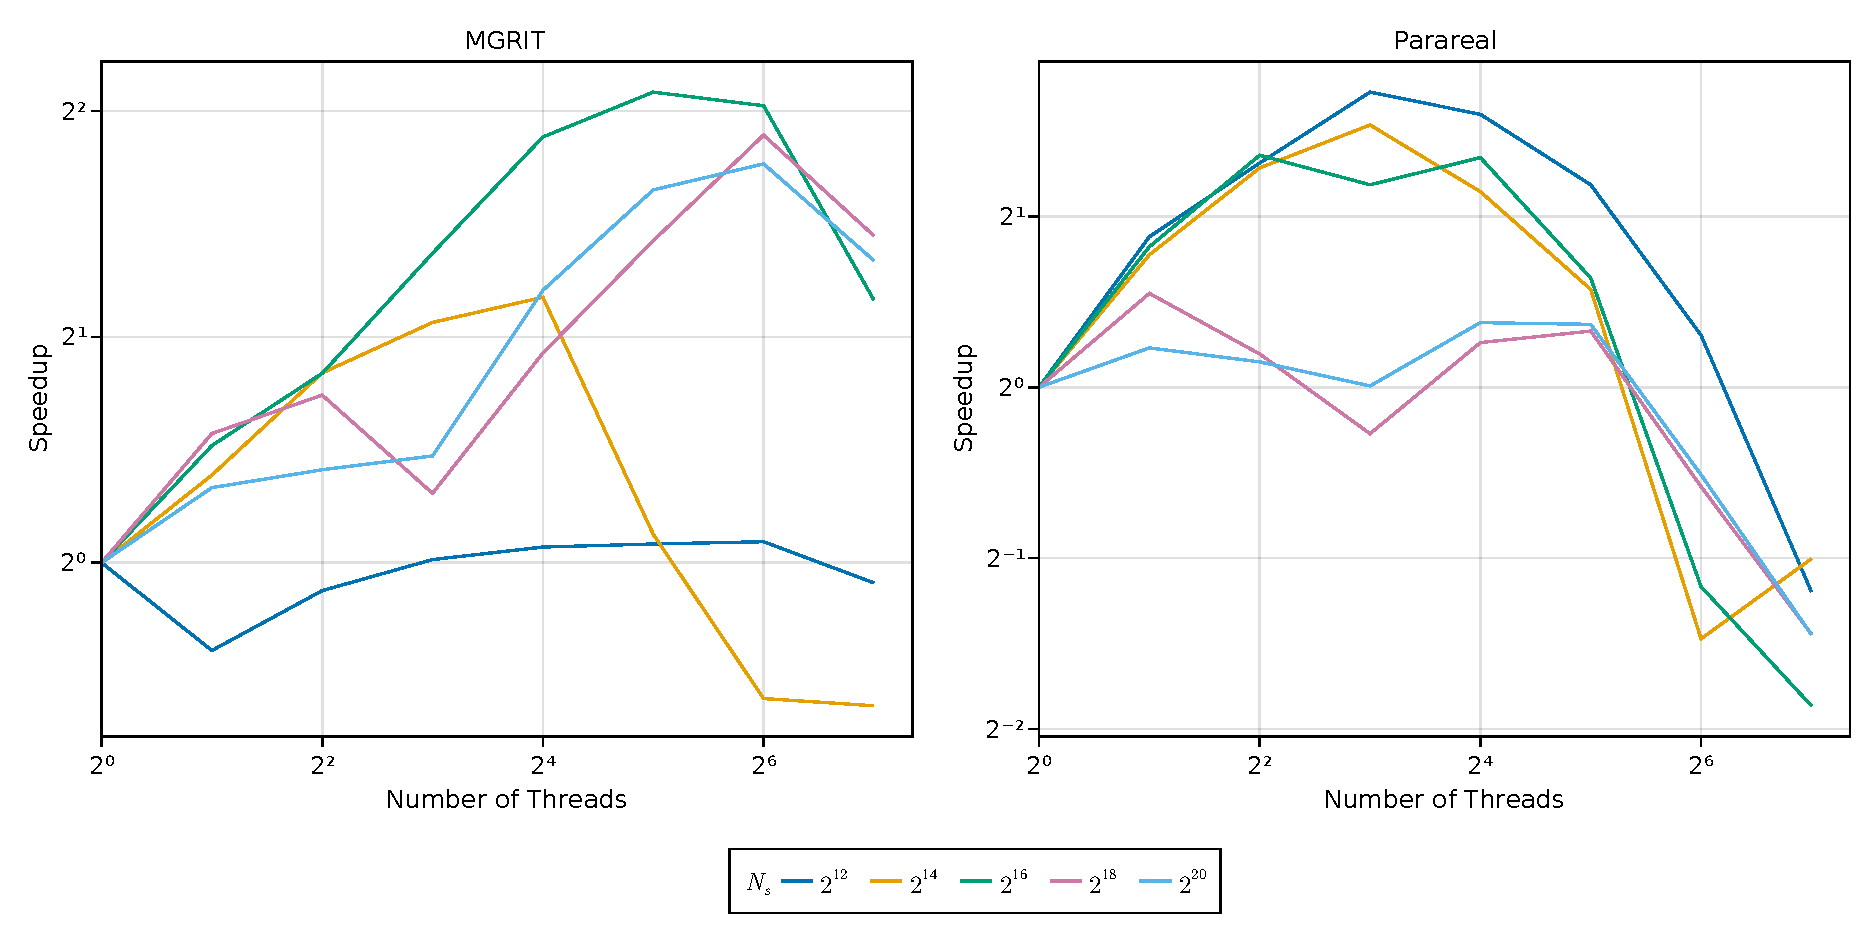
\includegraphics[width=\linewidth]{docs/assets/speedup_serial.pdf}
    \caption{Speedup of the MGRIT and Parareal Integrators relative to their performance with a single thread}
    \label{fig:heat_bench}
\end{figure}

As shown by Figure~\ref{fig:heat_bench}, both the MGRIT and Parareal integrators do show moderate speedups as the number of threads increases.
Due to the high cost of launching tasks using Julia's primitives (Section~\ref{sec:thread_overhead}), our speedup is highly dependent on problem size \(N_s\).
This is expected as the work per differential must be sufficiently large to cover the cost of launching tasks.
For MGRIT, it appears that \(N_s \geq 2^{16}\) is sufficient to support 64 threads as speedup continues to increase with the number of threads.
However for smaller problems \(N_s = 2^{14}\), above \~16 threads, the overhead of the additional threads outweighs the additional computing power.
Unfortunately, for small problems (\(N_s \leq 2^{12}\), the overhead of the threads virtually eliminates any speedup.

The hump shaped speedup curve of the Parareal integrator is a function of it's limitations as an integrator.
For low thread counts, the coarse integrator is able to quickly estimate a solution that is then refined by the fine integrator.
Resulting ina solution after only a few iterations.
However, as the thread count increases both the communication costs and task overhead increase linearly.
This results in the sudden drop in speedup with increasing thread count.
It is effectively similar to the drop in speedup observed for the MGRIT integrator, but occurs sooner, as the algorithmic advantage of more threads is less.

\begin{figure}[h]
    \centering
    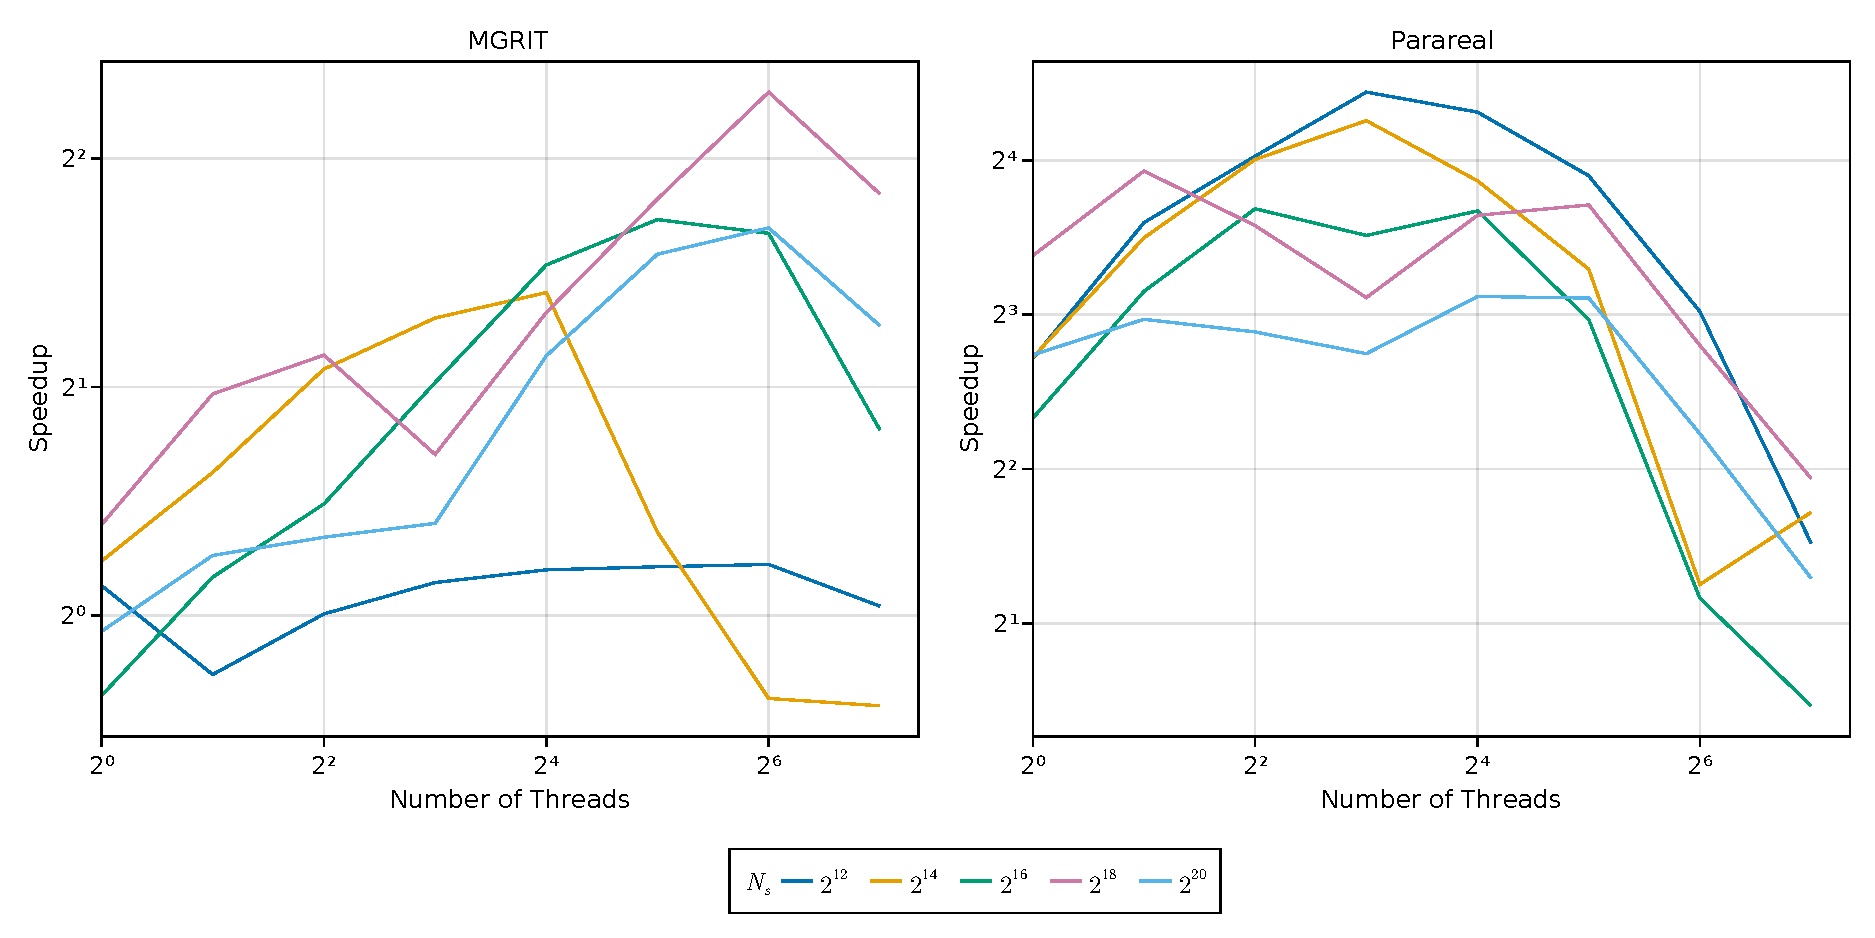
\includegraphics[width=\linewidth]{docs/assets/speedup_tsit5.pdf}
    \caption{Speedup of the MGRIT and Parareal Integrators relative to the performance of the Tsit5 integrator}
    \label{fig:heat_bench_tsit5}
\end{figure}

Both the MGRIT and Parareal algorithms were able to beat out the performance of the Tsit5 provided by DifferentialEquations.jl (Figure~\ref{fig:heat_bench_tsit5}).
This is a pleasant surprise, as the Tsit5 algorithm is DifferentialEquation.jl's recommended integrator for non-stiff problems\footnote{For the MATLAB Fans, while not exactly ode45, it is the recommended equivalent\cite{ODESolversDifferentialEquations}}.
Further, in benchmarks against other packages Tsit5 and DifferentialEquations.jl tend to beat out offerings~\cite{ODESolverMultiLanguage}.
That is, matching, let alone beating, the performance of the Tsit5 algorithm suggest that the parallel-in-time integration provided here provides a not insignificant value-add.

It should be noted that the performance of the Parareal over Tsit5 is likely in part due to the coarse integrator being allowed to make adaptive steps.
In effect this drastically reduces the cost of the coarse integrator, while retaining all of the benefits of the fine integrator.
Additionally, the Tsit5 integrator does save significantly more information (For example, it provides an accurate interpolant of the results), as well as suffering from run-time memory allocations as it does not pre-allocate space for the results.

\subsection{Profiling}

The next few pages show results from profiling the MGRIT algorithm on the 1D diffusion equation.
Profile was conducted using Julia's builtin statistical profiler, and visualized as a flamegraph using PProf.jl~\cite{PProfJl2022}.
Overall, similar trends to the benchmark results are observed, with larger problem sizes reducing the marginal cost of launching tasks.

\begin{landscape}
    \begin{figure}
        \centering
        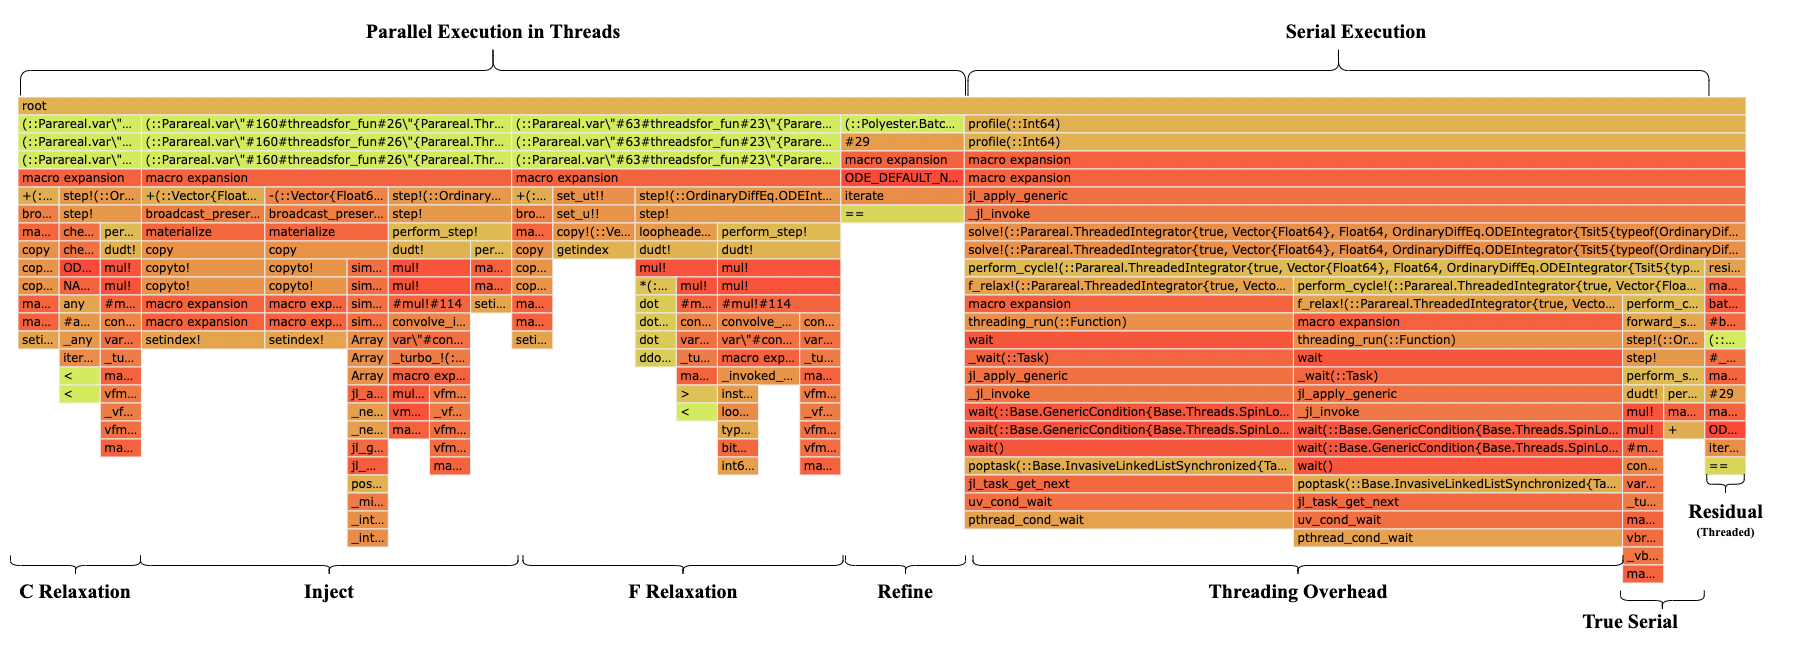
\includegraphics[width=\linewidth]{docs/assets/profile/profile_annotated.png}
        \caption{Annotated Flamegraph of MGRIT for a 1D Diffusion Equation with \(N_s = 2^{12}\) and \(N_t = 64\).
        As shown, threading overhead is significant and dominates the overall cost for small problem sizes.
        The Flamegraphs shown in Table~\ref{tab:sweep_profile} follow a similar trend, but with different proportions of work.
        Profiling occurred on an AMD EPYC 7713 64-Core Processor.
        }\label{fig:profile_annotated}
    \end{figure}
    \begin{table}
        \centering
        \begin{tabular}[t]{rccc}
            \(N_s\): & \(2^{12}\) & \(2^{16}\) & \(2^{20}\) \\
            \midrule
            \(N_t = 4\) &
                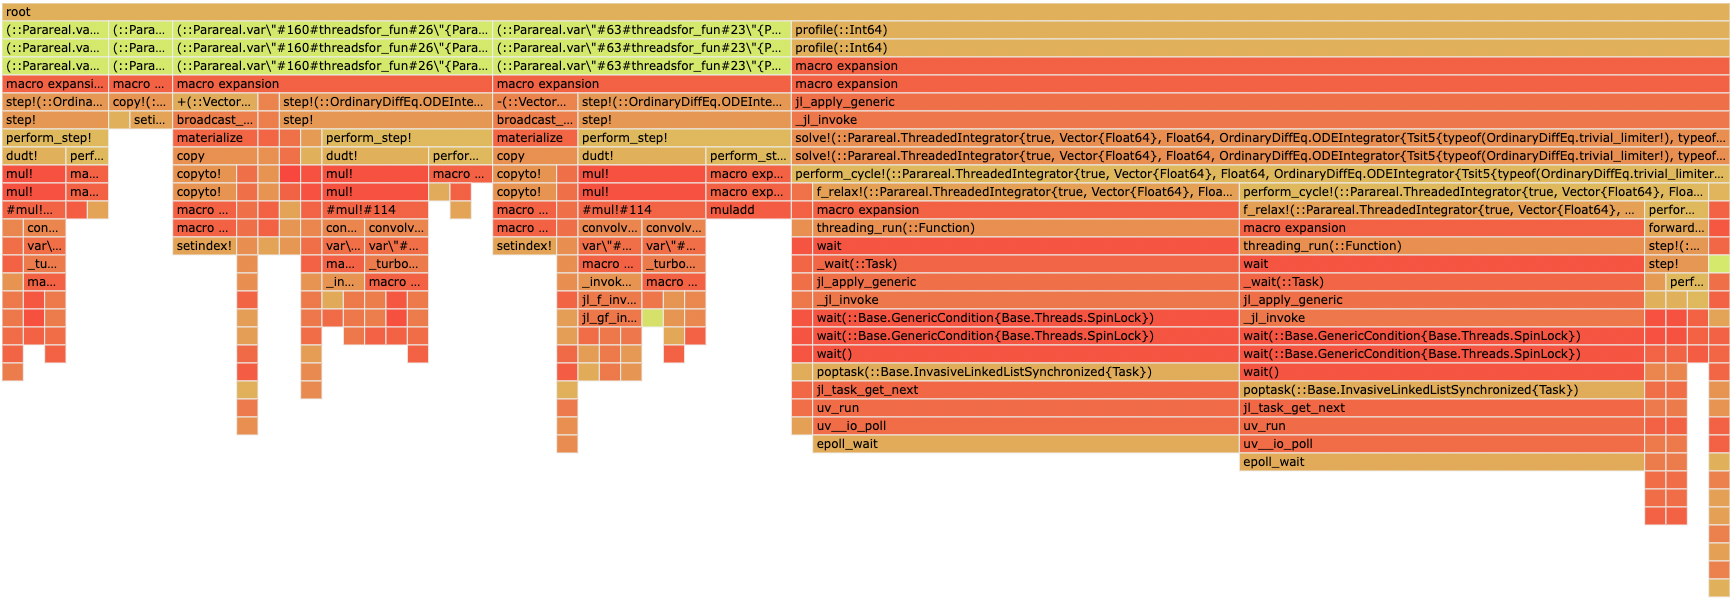
\includegraphics[width=.27\linewidth,valign=t]{docs/assets/profile/ns_12_nt_4.png} &
                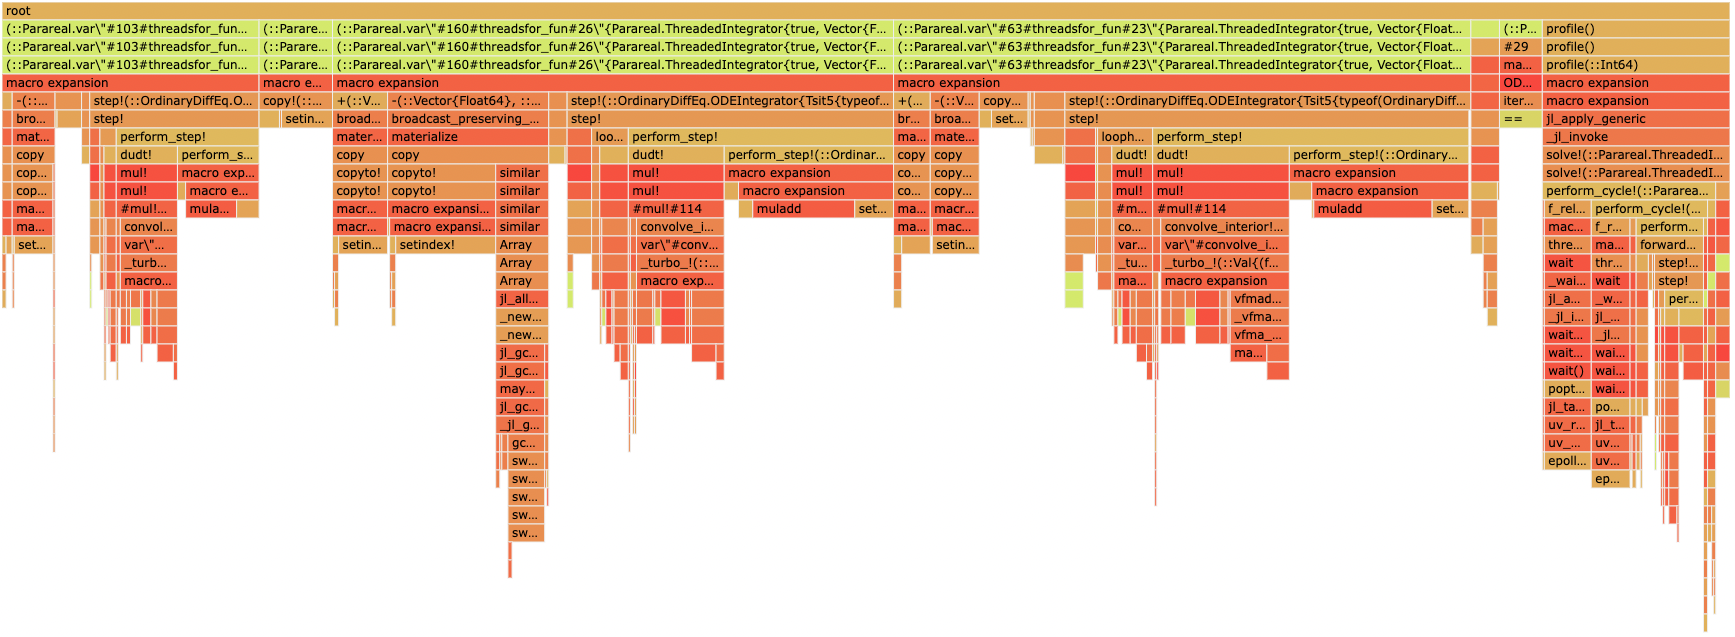
\includegraphics[width=.27\linewidth,valign=t]{docs/assets/profile/ns_16_nt_4.png} &
                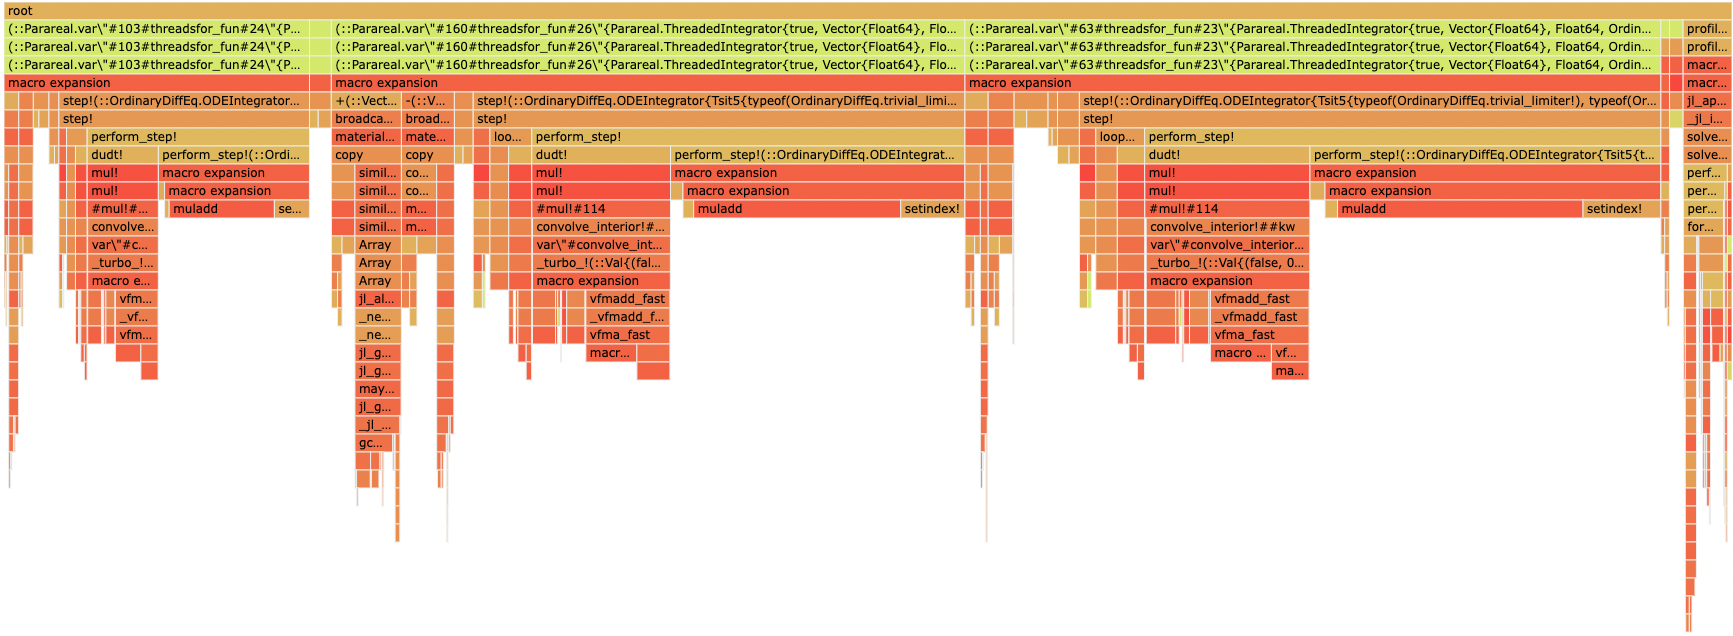
\includegraphics[width=.27\linewidth,valign=t]{docs/assets/profile/ns_20_nt_4.png} \\
            \(N_t = 16\) &
                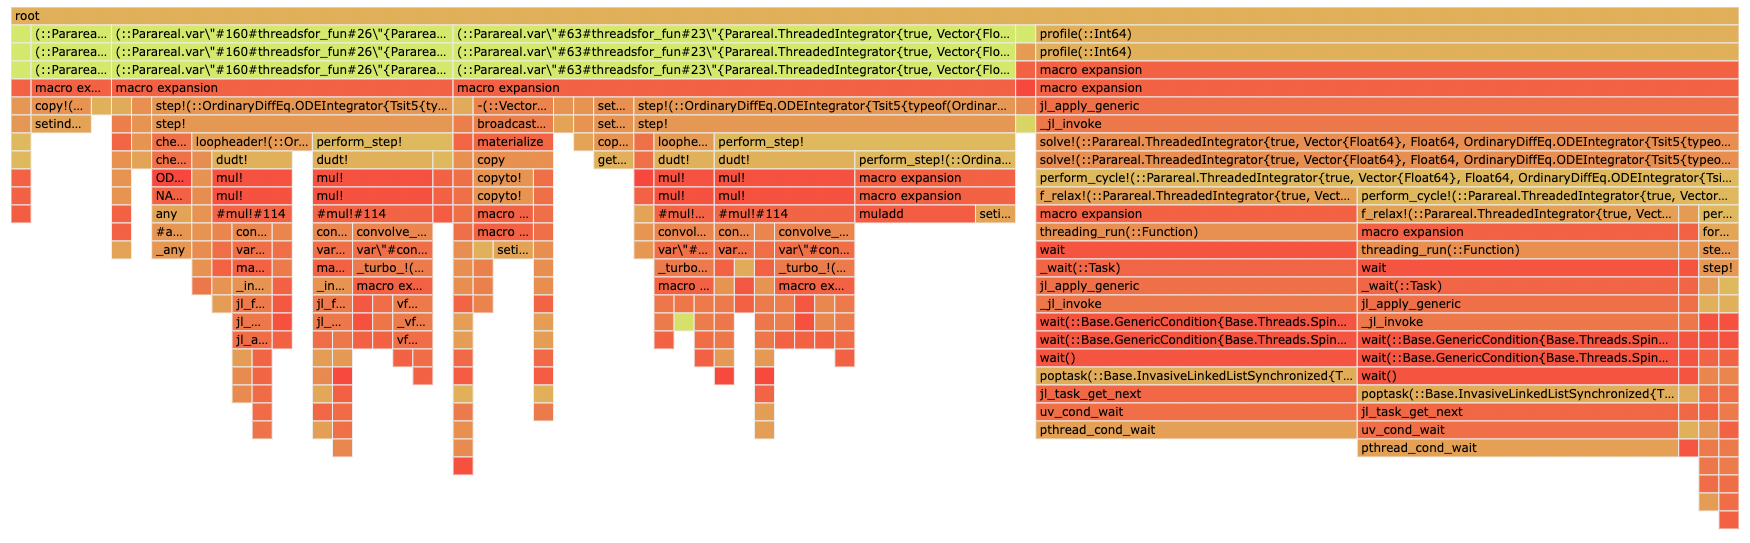
\includegraphics[width=.27\linewidth,valign=t]{docs/assets/profile/ns_12_nt_16.png} &
                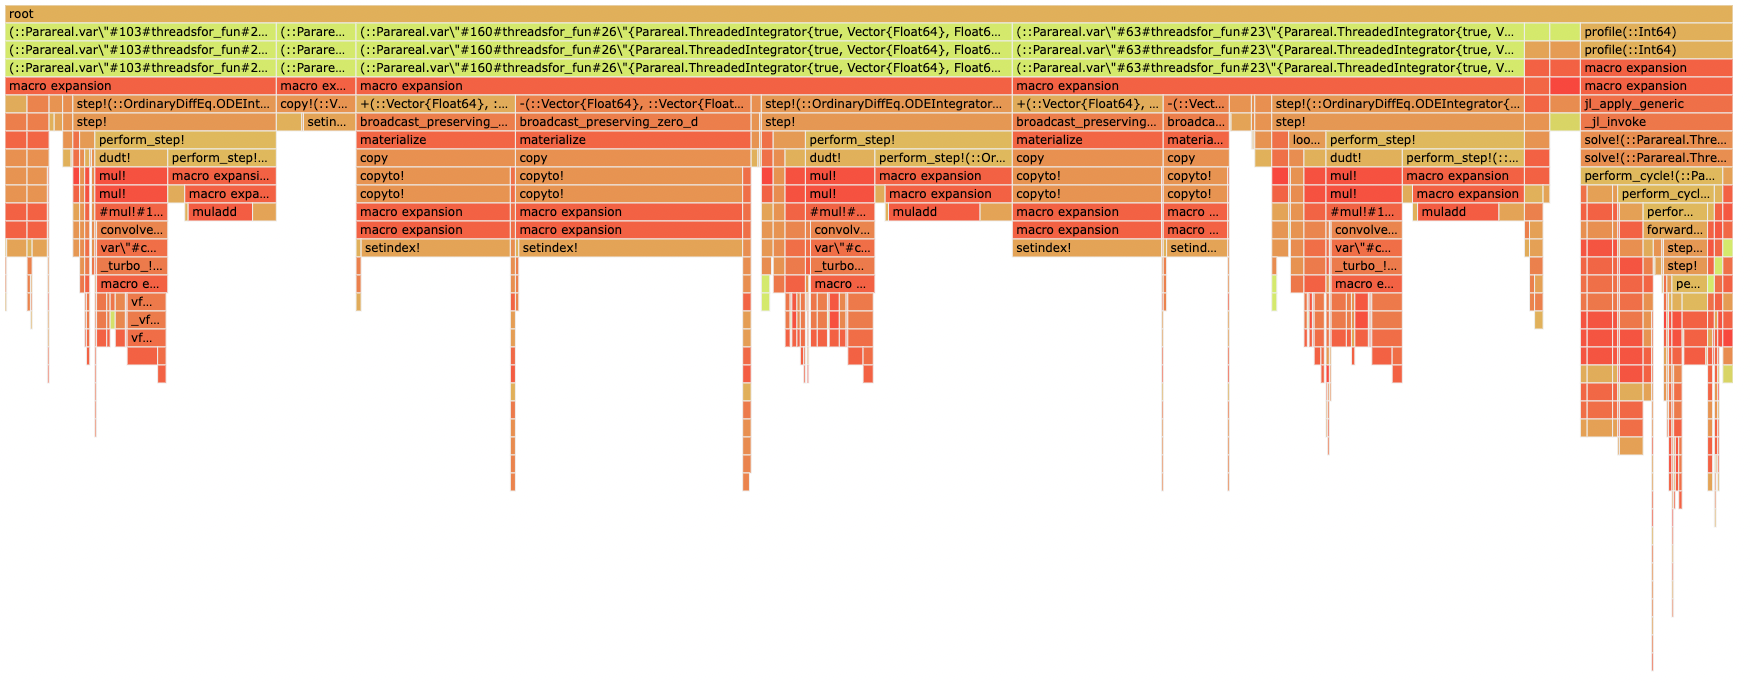
\includegraphics[width=.27\linewidth,valign=t]{docs/assets/profile/ns_16_nt_16.png} &
                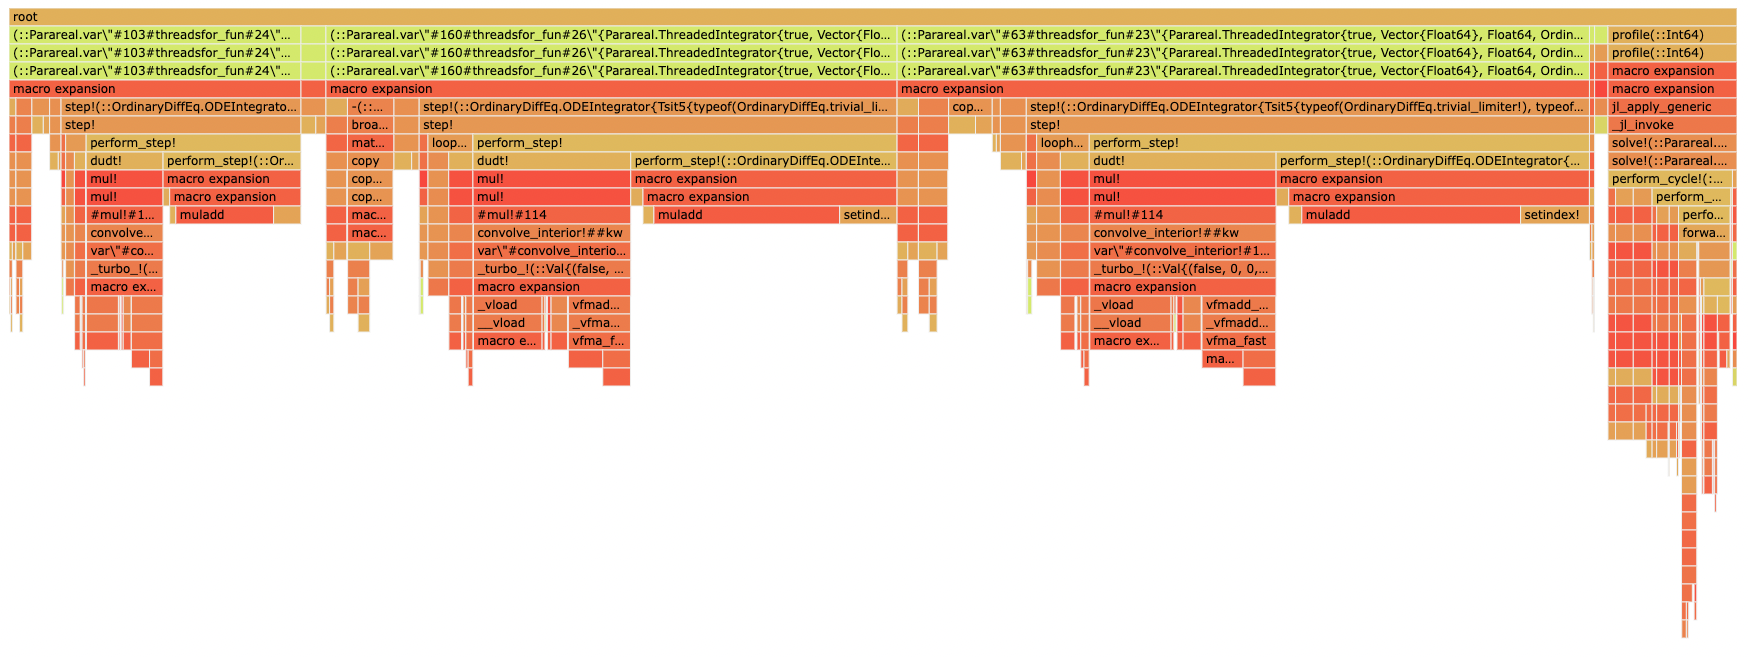
\includegraphics[width=.27\linewidth,valign=t]{docs/assets/profile/ns_20_nt_16.png} \\
            \(N_t = 64\) &
                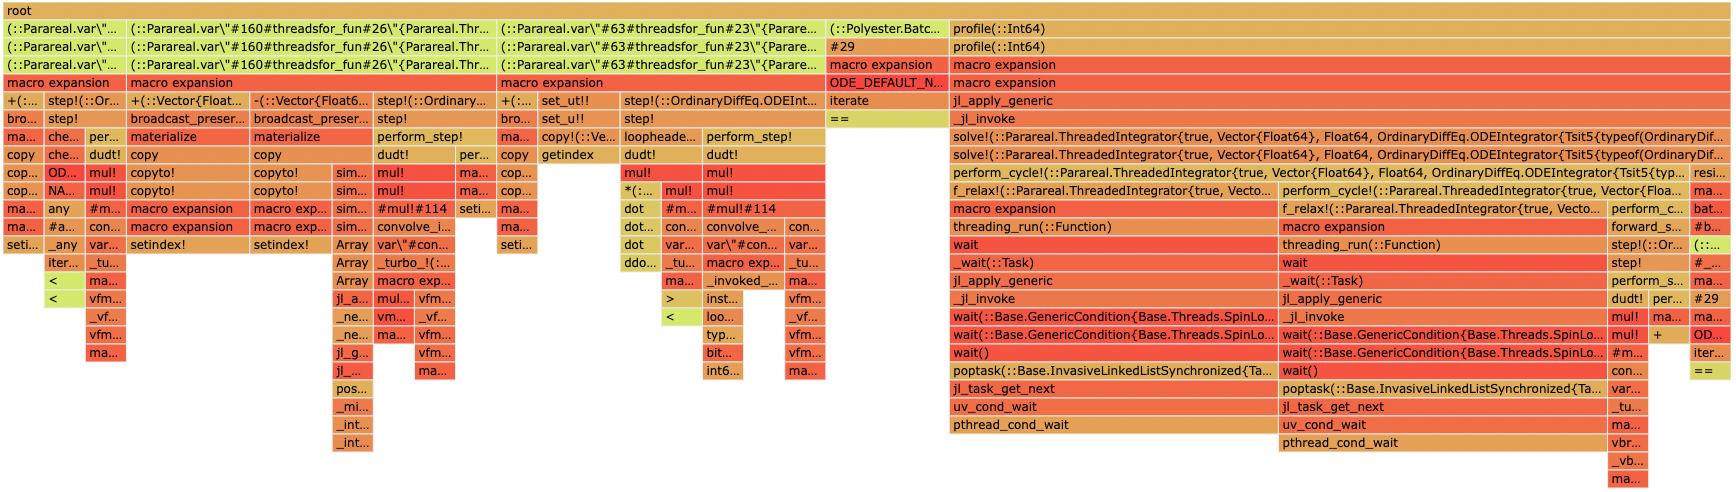
\includegraphics[width=.27\linewidth,valign=t]{docs/assets/profile/ns_12_nt_64.png} &
                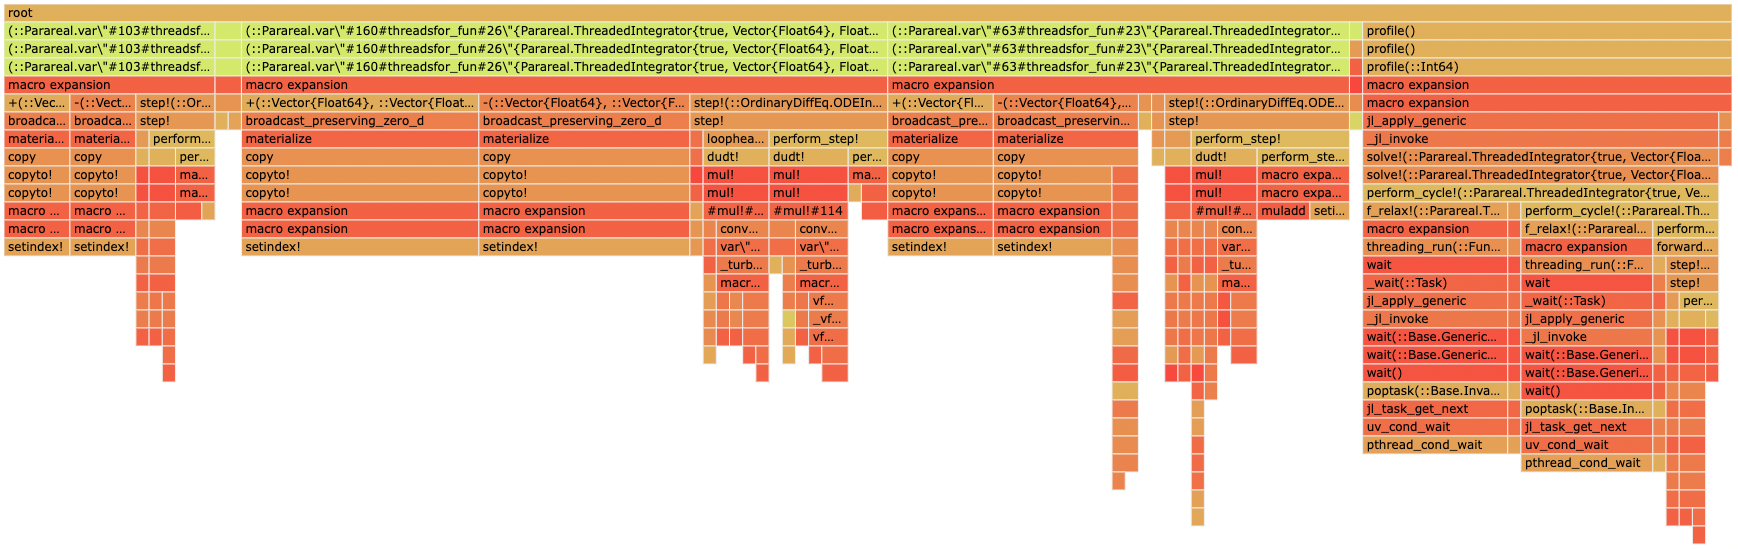
\includegraphics[width=.27\linewidth,valign=t]{docs/assets/profile/ns_16_nt_64.png} &
                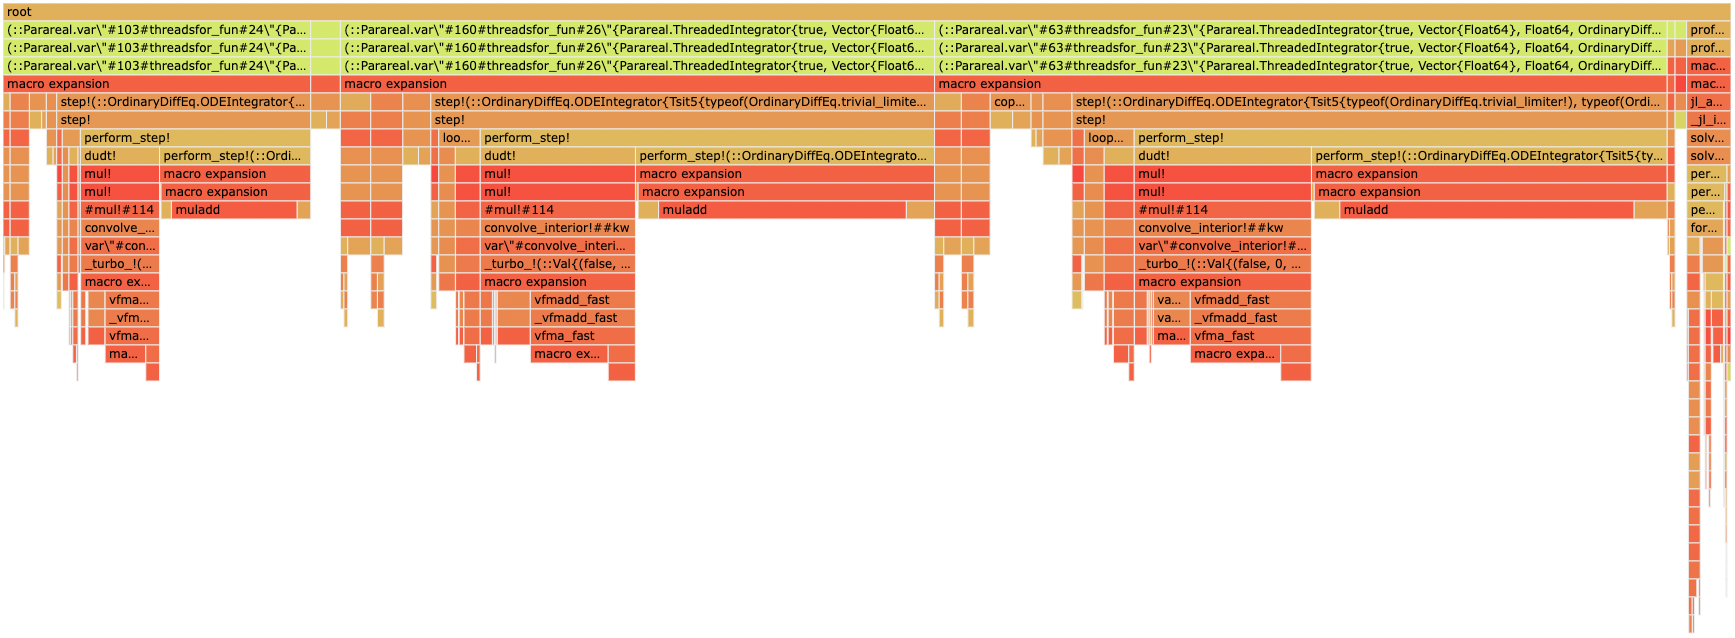
\includegraphics[width=.27\linewidth,valign=t]{docs/assets/profile/ns_20_nt_64.png} \\
            \bottomrule
        \end{tabular}
        \caption{Flamegraphs from profiling MGRIT on a 1D Diffusion Equation, while varying the work size \(N_s\) and number of threads \(N_t\).
        Profiling occurred on an AMD EPYC 7713 64-Core Processor.
        Overall, as work size increases, the overhead of launching threads becomes negligible, shrinking the serial execution region (See Figure~\ref{fig:profile_annotated} for a labeled flamegraph).
        As expected from the speedup plots (Figure~\ref{fig:heat_bench}), larger thread counts required a larger work size to effectively overcome the overhead of launching threads.
        }
        \label{tab:sweep_profile}
    \end{table}
\end{landscape}

\subsection{Working Set Size}
As shown in Figure~\ref{fig:heat_bench}, the \(N_s = 2^{20}\) performs worse than smaller work sizes, despite having
a generally higher level of parallelism (Table~\ref{tab:sweep_profile}).
While I was unable to confirm this via measurement with \verb!pref! due to noise from Julia's JIT compilation, I believe this is due to the cache size of the AMD EPYC 7713 processor.
With a state of \(2^n\) 64 bit floating point numbers, the total memory cost per time step is \((1 + 1/2 + 1/4 + 1/8) \times 8 \times 2^n \to 15 \times 2^n\) bytes.
Accounting for the 256 timesteps and 3x duplication of the state (\(u\), \(g\) and scratch space), this gives a total working set size of \(11520 \times 2^n\) bytes.
The maximum working set size the can fit into the L1, L2 or L3 caches of the AMD EPYC 7713 processor has be tabulated in Table~\ref{tab:cache_sizes}.

\begin{table}[h]
    \centering
    \begin{tabular}{rccc}
        Cache & Size [MiB] & Max \(N_s\) for single step & Max \(N_s\) for Entire Solution \\
        \midrule
        L1 & 4   & \(2^{16.5}\) & \(2^{8.5}\) \\
        L2 & 32  & \(2^{19.5}\) & \(2^{11.5}\) \\
        L3 & 256 & \(2^{22.5}\) & \(2^{14.5}\) \\
        \bottomrule
    \end{tabular*}
    \caption{Cache Sizes for the AMD EPYC 7713 Processor and maximum work sizes for a 1D Diffusion Equation.
        Cache sizes provided by WikiChip~\cite{EPYC7713AMD}.
    }\label{tab:cache_sizes}
\end{table}

As the working set size for a single time step at \(N_s = 2^{20}\) is larger than the L3 cache size, each core needs to access main memory to compute even a single timestep.
This results in the \(N_s = 2^{20}\) case having the lowest speedup with increasing thread counts due to increased contention for the main memory, and higher cache capacity misses.
This is further confirmed by the fact that the \(N_s = 2^{18}\) case saw the largest speedup overall (Figure~\ref{fig:heat_bench}).
As the working set for a single step can fit within the L2 cache, while the entire solution can fits within the L3 cache, when split across 64 cores.

\section{Future Work}

Given the results presented (Figure~\ref{fig:heat_bench}&\ref{fig:heat_bench_tsit5}), a Julia implementation of the MGRIT algorithm appears to be a viable contender for adding parallelism to the differential equation solver.
However, as noted above (Section~\ref{sec:thread_overhead}), the overhead of launching tasks is significant.
My choice to use Julia's threading primitives instead of it's distributed computing ones or an external package (i.e. MPI.jl) was largely motived by my use case: Accelerating solves on my personal laptop.
However, given the overhead of threads, and the tendency of MGRIT to require immense parallelism~\cite{friedhoffMULTIGRIDINTIMEALGORITHMSOLVING}, a message passing approach is likely to provide improved performance for sufficiently numerous computing resources.
This would also be in line with the approach taken by other implementations of the MGRIT algorithm~\cite{xbraid-package, hahnePyMGRITPythonPackage2020}.

Finally, as noted above (Section~\ref{sec:runtime_allocations}), my current implementation suffers from runtime memory allocations when resetting the serial integrators.
As the serial integrators provided by DifferentialEquations.jl are designed for serial solving of ODEs, they are not optimized for repeatedly being reset to a new initial condition.
Specifically, both the \verb!Euler! and \verb!Tsit5! integrators appear to re-allocate their internal caches when reset.
Further, performance could be achieved by eliminating these dynamic memory allocations.

Finally, while not pursued here, implementing the MGRIT algorithm on the GPU could provide access to the numerous execution units typically required~\cite{friedhoffMULTIGRIDINTIMEALGORITHMSOLVING}.
This concept was initially floated during my milestone update report, as I was not seeing any notable performance gains at the time.
However, by chasing down memory allocations and switching after implementing MGRIT, I was able to see a speedup a lower thread counts, thus eliminating the need for the massive (\(>2^{12}\) processor counts suggested by \citeauthor{friedhoffMULTIGRIDINTIMEALGORITHMSOLVING}, was no longer required.

\section{Work Distribution}

As this was a solo group project, all work was completed by Alex Wadell.

\clearpage
\printbibliography

\end{document}


